\documentclass[a4paper]{article}
\usepackage{amsmath,amssymb,amsfonts,amsthm}
\usepackage{multicol}
\usepackage{multirow}
\usepackage{mathtools}
\usepackage{soul}
\usepackage{hyperref}
\hypersetup{
    colorlinks=true,
    linkcolor=blue,
    filecolor=magenta,      
    urlcolor=cyan,
    pdftitle={Overleaf Example},
    pdfpagemode=FullScreen,
    }
\usepackage{color}
\usepackage[table]{xcolor}
\usepackage[T1]{fontenc}
\usepackage{etoolbox}
\usepackage{multicol}
\usepackage{multirow}
\usepackage{fancyhdr}
\usepackage{graphicx}
\usepackage{array}
\usepackage{amsthm}
\usepackage{titlesec}
\usepackage{tikz}
\usepackage{bm}
\usepackage{enumitem}
\usetikzlibrary{arrows.meta,calc}
\usetikzlibrary{positioning,automata}
\renewcommand{\baselinestretch}{1.2}

\titleformat*{\section}{\large\bfseries}
\titleformat*{\subsection}{\normalsize\bfseries}

\graphicspath{{C:/Users/teoso/OneDrive/Documents/Tugas Kuliah/Template Math Depart/}}

\newtheorem{theorem}{Theorem}
\newtheorem*{teorema}{Teorema}
\newtheorem*{definisi}{Definisi}
\theoremstyle{definition}
\newtheorem*{bukti}{Bukti}

\newcommand{\Arg}{\text{Arg}}

\begin{document}
\fancyhead[L]{\textit{Teosofi Hidayah Agung}}
\fancyhead[R]{\textit{5002221132}}
\pagestyle{fancy}
\section*{Exercise 2.1}
Perhatikan dua rangkaian perangkat keras berurutan berikut:

\begin{center}
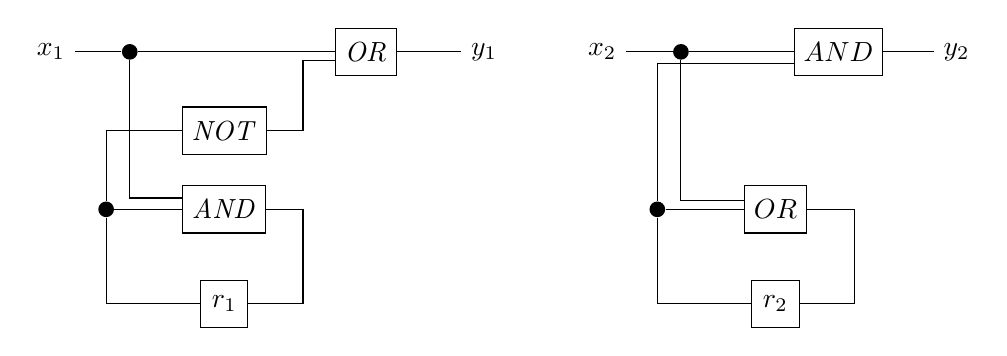
\begin{tikzpicture}[
  box/.style={draw, minimum width=0.6cm, minimum height=0.6cm},
  dot/.style={circle, fill, inner sep=2pt},
  node distance=1.5cm
  ]
  
  % First circuit on the left
  % Input
  \node (x1) at (0,0) {$x_1$};
  \node[dot, right of=x1, node distance=1cm] (dot1) {};
  \node[dot, below of=dot1, node distance=2cm,xshift=-0.3cm] (dot3) {};

  % Gates
  \node[box, right of=dot1, node distance=3cm] (or1) {\textit{OR}};
  \node[box, right of=dot3, node distance=1.5cm] (and1) {\textit{AND}};
  \node[box, above of=and1, node distance=1.0cm] (not1) {\textit{NOT}};
  \node[box, below of=and1, node distance=1.2cm] (r1) {$r_1$};
  
  % Output
  \node[right of=or1, node distance=1.5cm] (y1) {$y_1$};
  
  % Connections
  \draw (x1) -- (dot1);
  \draw (dot1) |- (and1.165);
  \draw (dot3) |- (and1);
  \draw (dot1) -- (or1);
  \draw (not1) -| (dot3);
  \draw (dot3) |- (r1);
  \draw (r1) -- ++(1,0) |- (and1);
  \draw (not1) -- ++(1,0) |- (or1.195);
  \draw (or1) -- (y1);
  
  % Second circuit on the right (shifted to the right)
  % Input
  \node (x2) at (7,0) {$x_2$};
  \node[dot, right of=x2, node distance=1cm] (dot2) {};
  \node[dot, below of=dot2, node distance=2cm,xshift=-0.3cm] (dot4) {};
  
  % Gates
  \node[box, right of=dot2, node distance=2.0cm] (and2) {$AND$};
  \node[box, right of=dot4, node distance=1.5cm] (or2) {$OR$};
  \node[box, below of=or2, node distance=1.2cm] (r2) {$r_2$};
  
  % Output
  \node[right of=and2, node distance=1.5cm] (y2) {$y_2$};
  
  % Connections
  \draw (x2) -- (dot2);
  \draw (dot2) -- (and2);
  \draw (dot2) |- (or2.165);
  \draw (dot4) -- (or2);
  \draw (dot4) |- (r2);
  \draw (dot4) |- (and2.195);
  \draw (r2) -- ++(1,0) |- (or2);
  \draw (and2) -- (y2);
    
\end{tikzpicture}
\end{center}
\noindent Dapatkan sistem transisi dari kedua rangkaian perangkat tersebut.\\

\noindent \textbf{Solusi:}\\
Pertama kita definisikan $\lambda_{y_1}, \lambda_{y_2}$ sebagai fungsi output dan $\delta_{r_1}, \delta_{r_2}$ sebagai fungsi transisi. Kemudian berdasarkan gambar di atas, karena rangkaian saling terpisahkan maka akan ditinjau masing-masing rangkaian.
\begin{enumerate}[label=(\arabic*)]
  \item Rangkaian pertama bergantung pada input $x_1$ dan $r_1$ dengan fungsi output $\lambda_{y_1}$ dan fungsi transisi $\delta_{r_1}$. Berdasarkan gambar, kita dapatkan informasi sebagai berikut:
  \begin{align*}
    \lambda_{y_1} &:= x_1 \lor \lnot r_1 \\
    \delta_{r_1} &:= x_1 \land r_1
  \end{align*}
  Kemudian \textit{state} awal untuk sistem transisi kita dapat didefinisikan 
  \[I:=\{\langle x_1=0, r_1=1 \rangle, \langle x_1=1, r_1=1 \rangle\}\]
  dan untuk setiap kemungkinan dapat diperoleh hasil-hasilnya sebagai berikut:
  \begin{align*}
    \langle x_1=0, r_1=1 \rangle &\longrightarrow \langle x_1=0, r_1=0 \rangle\\
    \langle x_1=0, r_1=1 \rangle &\longrightarrow \langle x_1=1, r_1=0 \rangle\\
    \langle x_1=1, r_1=1 \rangle &\longrightarrow \langle x_1=0, r_1=1 \rangle\\
    \langle x_1=1, r_1=1 \rangle &\longrightarrow \langle x_1=1, r_1=1 \rangle\\
    \langle x_1=0, r_1=0 \rangle &\longrightarrow \langle x_1=0, r_1=0 \rangle\\
    \langle x_1=0, r_1=0 \rangle &\longrightarrow \langle x_1=1, r_1=0 \rangle\\
    \langle x_1=1, r_1=0 \rangle &\longrightarrow \langle x_1=0, r_1=0 \rangle\\
    \langle x_1=1, r_1=0 \rangle &\longrightarrow \langle x_1=1, r_1=0 \rangle.
  \end{align*}
  Disisi lain tabel kebenaran untuk $\lambda_{y_1}$ adalah
  \begin{center}
    \begin{tabular}{|c|c|c|}
      \hline
      $x_1$ & $r_1$ & $\lambda_{y_1}$\\
      \hline
      0 & 0 & 1\\
      0 & 1 & 0\\
      1 & 0 & 1\\
      1 & 1 & 1\\
      \hline
    \end{tabular}
  \end{center}
  Sehingga sistem transisi dari rangkaian pertama dapat direpresentasikan sebagai berikut:
  \begin{center}
    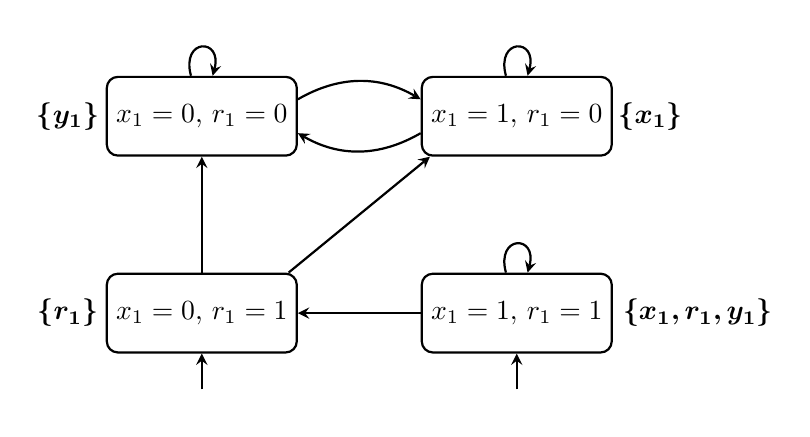
\begin{tikzpicture}[
      ->, >=stealth, node distance=2.5cm, on grid, thick,initial text=,
      state/.style={rectangle, rounded corners, draw, minimum width=2.0cm, minimum height=1cm},
      every loop/.style={looseness=3}]
  
      % Nodes
      \node[state] (q00) { $x_1 = 0,$  $r_1 = 0$ };
      \node[state, right=4cm of q00] (q10) { $x_1 = 1,$  $r_1 = 0$ };
      \node[state, below=of q00, initial below] (q01) { $x_1 = 0,$  $r_1 = 1$ };
      \node[state, below=of q10, initial below] (q11) { $x_1 = 1,$  $r_1 = 1$ };
  
      % Edges
      \path (q00.10) edge [bend left] node[above] {} (q10.170)
            (q10.-170) edge [bend left] node[above] {} (q00.-10)
            (q11) edge node {} (q01)
            (q00) edge[loop above] node {} ()
            (q10) edge[loop above] node {} ()
            (q11) edge[loop above] node {} ()
            (q01) edge node {} (q00)
            (q01.25) edge node {} (q10.-155)
            ;
      
      %Output
      \node[left=1.7cm of q00]  {$\bm{\{y_1\}}$};
      \node[left=1.7cm of q01]  {$\bm{\{r_1\}}$};
      \node[right=1.7cm of q10]  {$\bm{\{x_1\}}$};
      \node[right=2.3cm of q11]  {$\bm{\{x_1,r_1,y_1\}}$};
  
    \end{tikzpicture}
  \end{center}
  
  \item Rangkaian kedua bergantung pada input $x_2$ dan $r_2$ dengan fungsi output $\lambda_{y_2}$ dan fungsi transisi $\delta_{r_2}$. Berdasarkan gambar, kita dapatkan informasi sebagai berikut:
  \begin{align*}
    \lambda_{y_2} &:= x_2 \land r_2 \\
    \delta_{r_2} &:= x_2 \lor r_2
  \end{align*}
  Kemudian \textit{state} awal untuk sistem transisi kita dapat didefinisikan 
  \[I:=\{\langle x_2=0, r_2=0 \rangle, \langle x_2=1, r_2=0 \rangle\}\]
  dan untuk setiap kemungkinan dapat diperoleh hasil-hasilnya sebagai berikut:
  \begin{align*}
    \langle x_2=0, r_2=0 \rangle &\longrightarrow \langle x_2=0, r_2=0 \rangle\\
    \langle x_2=0, r_2=0 \rangle &\longrightarrow \langle x_2=1, r_2=0 \rangle\\
    \langle x_2=1, r_2=0 \rangle &\longrightarrow \langle x_2=0, r_2=1 \rangle\\
    \langle x_2=1, r_2=0 \rangle &\longrightarrow \langle x_2=1, r_2=1 \rangle\\
    \langle x_2=0, r_2=1 \rangle &\longrightarrow \langle x_2=0, r_2=1 \rangle\\
    \langle x_2=0, r_2=1 \rangle &\longrightarrow \langle x_2=1, r_2=1 \rangle\\
    \langle x_2=1, r_2=1 \rangle &\longrightarrow \langle x_2=0, r_2=1 \rangle\\
    \langle x_2=1, r_2=1 \rangle &\longrightarrow \langle x_2=1, r_2=1 \rangle.
  \end{align*}
  Disisi lain tabel kebenaran untuk $\lambda_{y_2}$ adalah
  \begin{center}
    \begin{tabular}{|c|c|c|}
      \hline
      $x_2$ & $r_2$ & $\lambda_{y_2}$\\
      \hline
      0 & 0 & 0\\
      0 & 1 & 0\\
      1 & 0 & 0\\
      1 & 1 & 1\\
      \hline
    \end{tabular}
  \end{center}
  Sehingga sistem transisi dari rangkaian kedua dapat direpresentasikan sebagai berikut:
  \begin{center}
    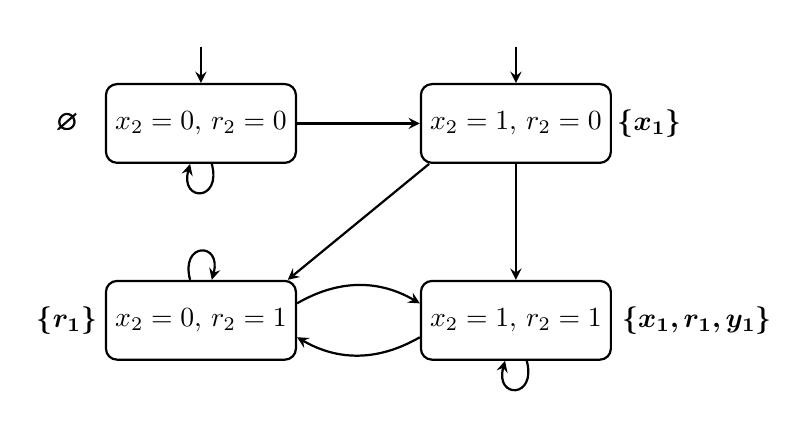
\begin{tikzpicture}[
      ->, >=stealth, node distance=2.5cm, on grid, thick,initial text=,
      state/.style={rectangle, rounded corners, draw, minimum width=2.0cm, minimum height=1cm},
      every loop/.style={looseness=3}]
  
      % Nodes
      \node[state, initial above] (q00) { $x_2 = 0,$  $r_2 = 0$ };
      \node[state, initial above, right=4cm of q00] (q10) { $x_2 = 1,$  $r_2 = 0$ };
      \node[state, below=of q00] (q01) { $x_2 = 0,$  $r_2 = 1$ };
      \node[state, below=of q10] (q11) { $x_2 = 1,$  $r_2 = 1$ };
  
      % Edges
      \path (q00) edge[loop below] node {} ()
            (q00) edge node {} (q10)
            (q10.-155) edge node {} (q01.25)
            (q10) edge node {} (q11)
            (q01) edge[loop above] node {} ()
            (q01.10) edge[bend left] node {} (q11.170)
            (q11.-170) edge[bend left] node {} (q01.-10)
            (q11) edge[loop below] node {} ();
            ;
      
      %Output
      \node[left=1.7cm of q00]  {$\bm{\varnothing}$};
      \node[left=1.7cm of q01]  {$\bm{\{r_1\}}$};
      \node[right=1.7cm of q10]  {$\bm{\{x_1\}}$};
      \node[right=2.3cm of q11]  {$\bm{\{x_1,r_1,y_1\}}$};
  
    \end{tikzpicture}
  \end{center}
\end{enumerate}
  
\end{document}